\documentclass{article}[10pt]
\usepackage{graphicx}
\usepackage{xspace}
\usepackage{url}
\usepackage{listings}
\usepackage{color}

\definecolor{pblue}{rgb}{0.13,0.13,1}
\definecolor{pgreen}{rgb}{0,0.5,0}
\definecolor{pred}{rgb}{0.9,0,0}
\definecolor{pgrey}{rgb}{0.46,0.45,0.48}

\lstset{language=Java,
  showspaces=false,
  showtabs=false,
  breaklines=true,
  showstringspaces=false,
  breakatwhitespace=true,
  commentstyle=\color{pgreen},
  keywordstyle=\color{pblue},
  stringstyle=\color{pred},
  basicstyle=\ttfamily,
  moredelim=[il][\textcolor{pgrey}]{$$},
  moredelim=[is][\textcolor{pgrey}]{\%\%}{\%\%}
}

\newcommand{\lstJava}[1]{\lstinline[language=Java,breaklines=true,mathescape,literate={\-}{}{0\discretionary{-}{}{}}]�#1�}
\newcommand{\tapcli}{Tapestry5-cli\xspace}

\begin{document}

\title{\tapcli Library}
\author{Alessio Gambi}

\maketitle

\begin{abstract}
This document briefly describes the design process of the \tapcli.
The idea is to illustrate over a real example how to design new services for the framework, and ideally, start sketching a generic process to develop Tapestry5 applications.
\end{abstract}

\section{Introduction}

\section{The Problem}
We need to parse the command line input of our programs, check its validity, and make the various options and inputs available to the application.
If the parsing or the validation fail we need to print on the console an error message, what failed and why, and a usage message.

All the messages must be localized. Error messages must be as specific as possible, while the usage message must list all the available components.

We want to configure the library in a distributed fashion: Components defined in different modules can contribute their own input options, and configurations.
In the spirit of Tapestry, validation mechanisms, messages, and all the other contributions can be specified as well.

\section{Solution Overview}
We want to exploit Tapestry5-IoC to design a library that provide a service, called \lstJava{CLIParser}, that receives all the contributions, implement the parsing and the validation of the command line input.

On one side, we rely on predefined CLI parsing libraries, such as commons-cli by Apache\footnote{\url{http://commons.apache.org/proper/commons-cli/}}, for the parsing side, and Tapestry services for validation and messaging. 
%
We use the distributed configuration feature of Tapestry to collect all the user provide configuration and configure the third-party libraries, the validation framework, and so on.

Figure~\ref{fig:overview} depicts an informal overview of the solution: the \lstJava{CLIParser} service receives the input arguments, try to parse them using an injected {\em Parsing} service that is pipelined with the {\em Validation} service. If the parsing succeeds the control passes to the validation, otherwise a Parsing exception is raised and the pipeline breaks. Similarly, if the validation succeeds the control pass over, otherwise a Validation exception is raised and the pipeline breaks. Eventually, the library exports the validated inputs as symbols to be accessed elsewhere in the application.

\begin{figure}
 \centering
  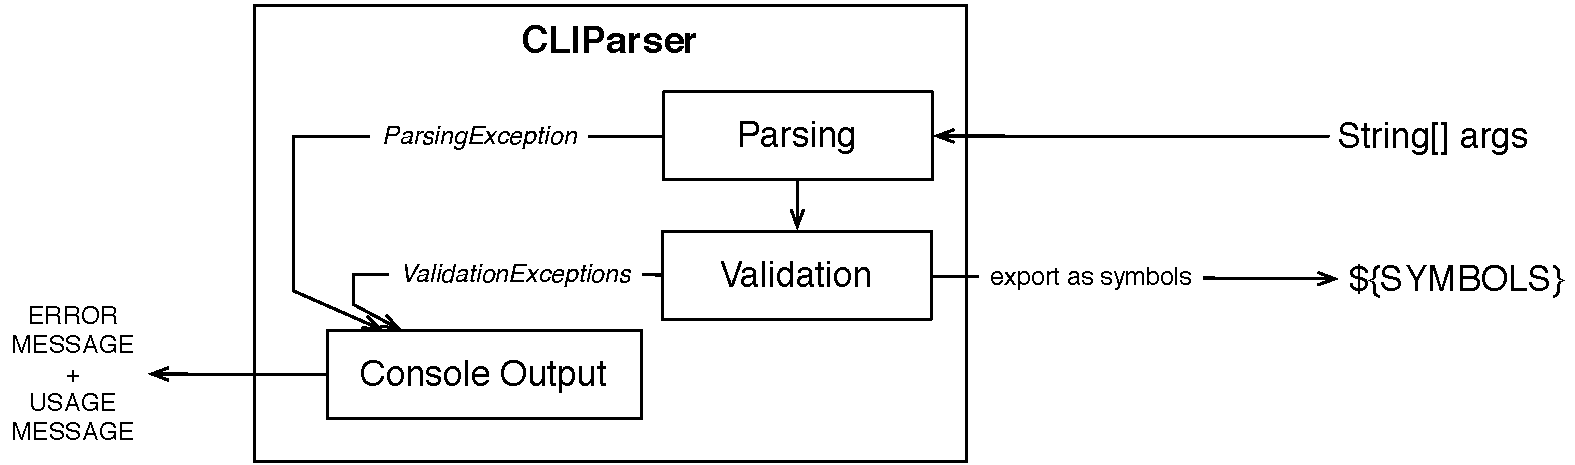
\includegraphics[width=0.8\textwidth]{figs/overview.pdf}
  \caption{Overview of the tapestry5-cli library}
  \label{fig:overview}
\end{figure}

\subsection*{Architectural considerations and design alternatives}

The previous description suggests that a possible design patterns to be used here is the Chain-of-Command, where the default command is the one that exports all its input arguments (a variable number of \lstJava{\<String,String\>} entries) as symbols, like a \lstJava{SymbolSource}. Parsing and validation are additional commands injected before this one.
%
Under this light we can think of different alternatives:

\begin{description}
\item[Mock Up Requests] One solution is to mock up the startup process as a single request to the framework, and exploits as much as possible the services already available in the framework, as well as their organization. 

\item[Create a clone of the  Request Pipeline] Another way to reuse as much as possible the services already defined is to recreate the main pipeline request process. In this way, we can choose what service to put inside the pipeline processing and we limit the `hacking' of having a non-web request processed as a web-one.

\item[Implement the service from scratch] Instead of replicating tapestry code we can build one own service from scratch, meaning that we can organize the \lstJava{SymbolProvider}, the parsing and the validation services ``manually''.

\end{description}

\section{Details on the various alternatives solution}

\subsection*{}


\section{Conclusion}


\end{document}